\documentclass[11pt,leqno]{article}
\usepackage[T1]{fontenc}
\usepackage{amsmath}%
\usepackage{amsthm}
\usepackage{amsxtra}%
\usepackage{amsfonts}%
\usepackage{amssymb}%
\usepackage[margin=1in]{geometry}
\usepackage{color,hyperref}
\usepackage{graphicx}
\usepackage{subfig}
\usepackage{cite}
\hypersetup{colorlinks,breaklinks,
             linkcolor=blue,urlcolor=blue,
             anchorcolor=blue,citecolor=blue}
\usepackage{color}
\usepackage{array}
\usepackage{booktabs}

%\usepackage{showlabels}
\newcommand{\iid}{\emph{i.i.d.}}
\newcommand{\coti}{\text{cot}^{-1}}
\newcommand{\A}{{\mathcal A}}
\renewcommand{\O}{{\mathcal O}}
\renewcommand{\bar}[1]{{\overline{#1}}}
\newcommand{\F}{{\mathcal F}}
\renewcommand{\P}{{\mathcal P}}
\newcommand{\X}{{\mathcal X}}
\renewcommand{\H}{{\mathcal H}}
\newcommand{\R}{\mathbb{R}}
\newcommand{\N}{\mathbb{N}}
\newcommand{\Q}{\mathbb{Q}}
\newcommand{\No}{\mathbb{N}_0}
\newcommand{\Z}{\mathbb{Z}}
\newcommand{\vb}[1]{\mathbf{#1}}
\newcommand{\supp}{{\rm supp}}
\newcommand{\eps}{\varepsilon}
\renewcommand{\tilde}[1]{\widetilde{#1}}
\renewcommand{\phi}{\varphi}
\newcommand{\limsupn}{\limsup_{n\to \infty}}
\newcommand{\liminfn}{\liminf_{n\to \infty}}
\newcommand{\limn}{\lim_{n\to \infty}}
\newcommand{\ppp}[1]{\Pi_{#1}}
\newcommand{\spn}{\text{span}}
\newcommand{\adj}{\text{Adj}}
\newcommand{\curl}{\text{curl}}
\renewcommand{\div}{\text{div}}
\renewcommand{\S}{\mathbb{S}}
\def\Xint#1{\mathchoice
{\XXint\displaystyle\textstyle{#1}}%
{\XXint\textstyle\scriptstyle{#1}}%
{\XXint\scriptstyle\scriptscriptstyle{#1}}%
{\XXint\scriptscriptstyle\scriptscriptstyle{#1}}%
\!\int}
\def\XXint#1#2#3{{\setbox0=\hbox{$#1{#2#3}{\int}$ }
\vcenter{\hbox{$#2#3$ }}\kern-.6\wd0}}
\def\ddashint{\Xint=}
\def\dashint{\Xint-}

\newcommand{\heading}[1]{\vspace{10pt}\noindent{\bf #1:}}
\newtheorem{theorem}{Theorem}
\newtheorem{lemma}[theorem]{Lemma}
\newtheorem{corollary}[theorem]{Corollary}
\newtheorem{example}{Example}
\newtheorem{proposition}[theorem]{Proposition}
\theoremstyle{definition}
\newtheorem{remark}[theorem]{Remark}
\newtheorem{definition}[theorem]{Definition}
\newtheorem{problem}[theorem]{Problem}
\newtheorem{conjecture}[theorem]{Conjecture}

\newcommand{\vg}{\smash{\includegraphics[height=11pt]{virtual_goniometer}}\;}
\renewcommand{\next}{\smash{\includegraphics[height=11pt]{virtual_goniometer_next}}\;}
\newcommand{\reset}{\smash{\includegraphics[height=11pt]{virtual_goniometer_reset}}\;}
\newcommand{\undo}{\smash{\includegraphics[height=11pt]{virtual_goniometer_undo}}\;}
\newcommand{\select}{\smash{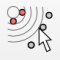
\includegraphics[height=11pt]{Select}}\;}

\title{Blender Plugin Documentation}
\author{Paige Cody \\ \url{cody0041@umn.edu}}
%
\begin{document} 
\maketitle

This documentation describes the AMAAZE Blender plugin: The virtual goniometer.

\section{Virtual Goniometer}

The virtual goniometer plugin can be used to take angle measurements on triangulated meshes. Each section below describes basic features of Blender and how to use the plugin. For more details on the plugin, see our paper\dots

\subsection{Installing the Blender plugin}

The plugin is currently available on Github \url{https://github.com/paigeco/VirtualGoniometer.git}. To install the plugin, navigate to Edit -> Preferences -> Add-ons -> Install and then select and enable the Virtual Goniometer from the menu. More detailed installation instructions can be found on the download page.
\begin{figure}
\centering
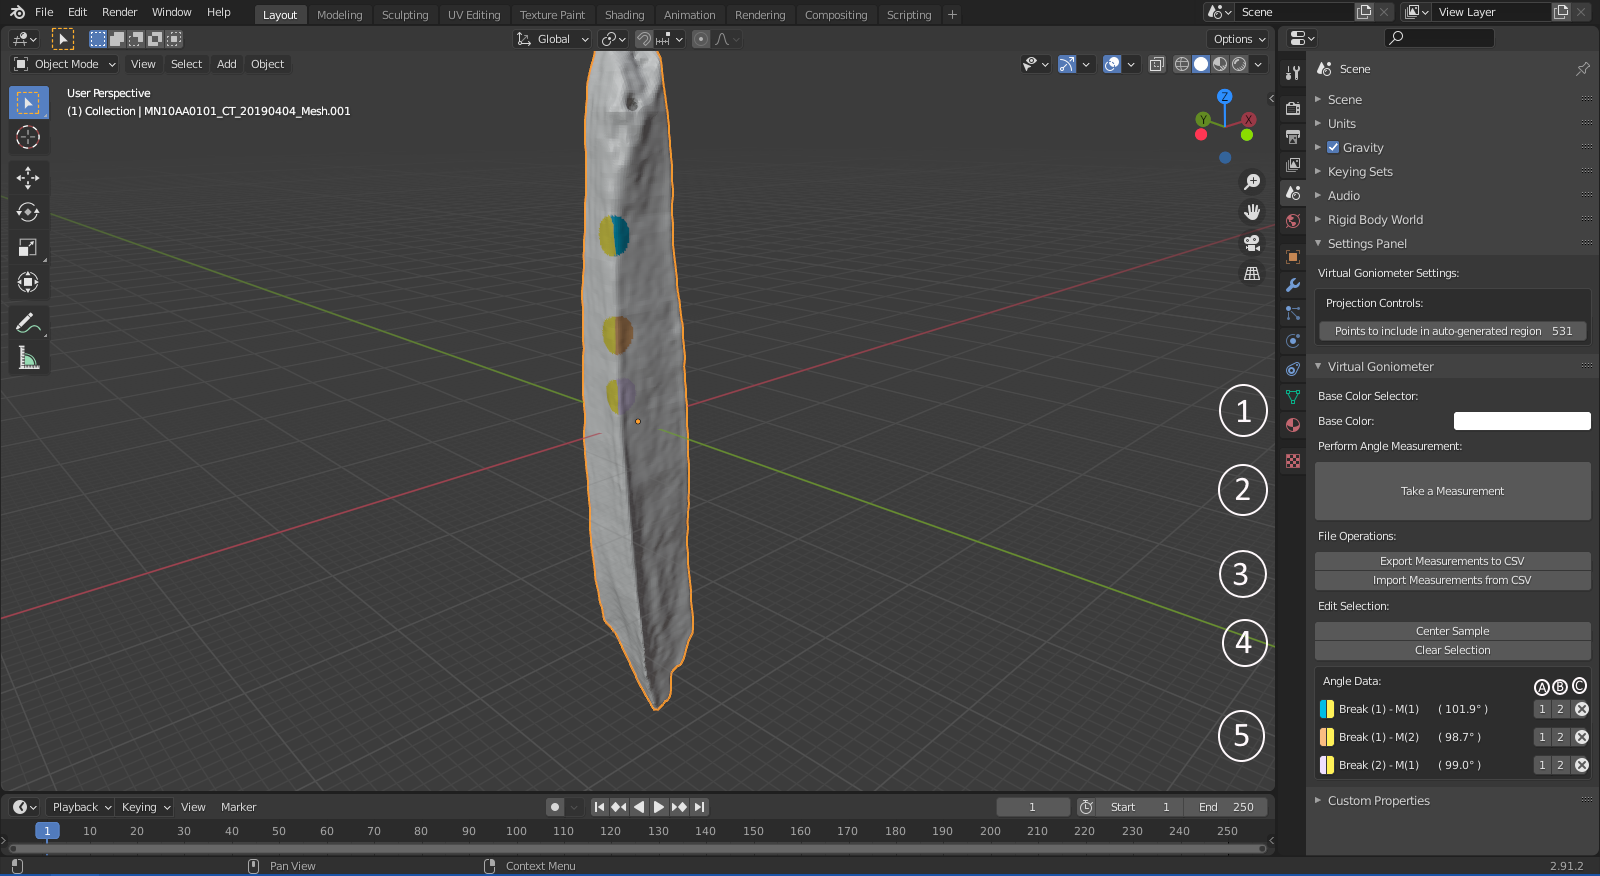
\includegraphics[width=0.9\textwidth]{VG_Menu.png}
\caption{Virtual Goniometer.}
\label{fig:VG_Menu}
\end{figure}
\subsection{Taking Measurements \texorpdfstring{\select}{select}}


To run the Virtual Goniometer the user must first import and select a mesh to make measurements on. This can be done using the included Blender importer located in File -> Import. To begin taking measurements, the user must navigate to the "Virtual Goniometer" panel located in the Properties -> Scene window as seen in Figure \ref{fig:VG_Menu}. To take a measurement, the user must click the "Take a Measurement button seen near (2). Once the button has been clicked, the measurement routine will begin. Each the time the measurement routine is begun the specific instance will be assigned its own "Break Number" sequentially. To select a location to be used as the center of a measurement, Left-Click on the desired area and the measurement will be saved to the "Angle Data" field near (5). To orbit around the object hold the Middle-Click button and move the mouse, to pan around the object hold both Middle-Click and shift and move the mouse. When the measurements have been completed, Right-Click to end the measurement routine.


\subsection{Editing a Measurement}
\begin{figure}
\centering
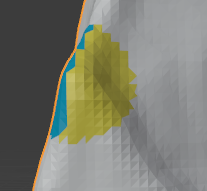
\includegraphics[width=0.2\textwidth]{Edit 1.PNG}
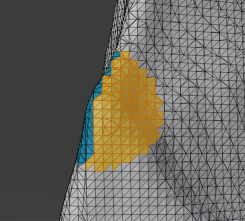
\includegraphics[width=0.2\textwidth]{Edit 2.PNG}
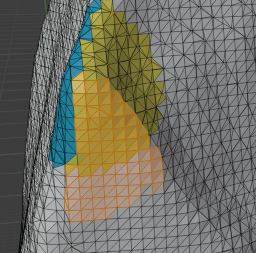
\includegraphics[width=0.2\textwidth]{Edit 3.PNG}
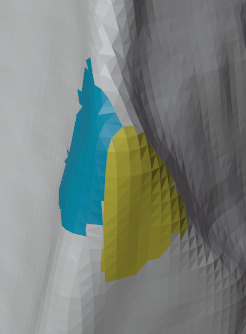
\includegraphics[width=0.2\textwidth]{Edit 4.PNG}
\caption{The process of using the Edit Side function to solve a strange segmentation.}
\label{fig:VG_EditExample}
\end{figure}

The "Angle Data" section of the Virtual Goniometer shown near (5) in Figure \ref{fig:VG_Menu} contains a row for each measurement made as well as buttons which allow for editing certain aspects of the measurements. From left to right these functions are.
\begin{itemize}
\item {\bf Color Selector:} If the user desires to change from the default colors, they can click on the color which they desire to change. This employs a pop-up color wheel which allows for users to select unique identifying colors for their measurements as is seen in Figure \ref{fig:VG_ColorSelector}.
\item {\bf Break and Measurement Index:} The next field shows both the break and measurement numbers of the object in question.
\item {\bf Angle Measured:} This field shows the measured angle between the two faces shown in degrees.
\item {\bf Side 1/2 Editing:} These two buttons allow for the editing of Side 1/2 respectively illustrated by the colors shown at the beginning of the row. By clicking on one of the buttons, the respective side will be brought into "Edit-Mode" and individual faces can then be removed or added to the face included in the measurement. The faces highlighted in orange will be saved to the side. Using Ctrl-C will allow the user to get a circle select tool which adds to the region with Left-Mouse and removes from the region with Right-Mouse. When the user is done, they merely have push the same button again to confirm the changes to the side. An example of how this can be used is shown in Figure \ref{fig:VG_EditExample}
\end{itemize}


\subsection{CSV File Input-Output}

All angle measurements taken in the plugin can be saved to a CSV file using the "Export Measurements to CSV" function located under "File Operations:". The file contains a lot of information about the measurements, including the mesh name, date and time the measurement was taken, break \# and measurement \#, colors used to indicated clustering, angle, radius of the patch, number of vertices in the patch, and the center point of the patch. Once the function is run, the user will be prompted to enter the path to save the file to. Angles for a given break can also be loaded from a CSV file using the "Import Measurements form CSV" function also located in "File Operations". Once saved, the file will no longer update, so make sure to save often!


%\subsection{Undo a measurement}

%The plugin has an \verb|undo| feature, which is run via the shortcut key \verb|Ctrl+Z|. There is no %redo feature so be careful!

\subsection{Clear and Center\texorpdfstring{\clear}{clear}}

The "Center Sample" and the "Clear Selection" buttons (as seen in Figure \ref{fig:VG_Menu} near (4)) are both options which are included for the convenience of the user.\\

The "Center Sample" button merely centers the object in the blender work area to the point (0,0,0) in three dimensional space. It can be very helpful due to occasional large spacial offsets from the center of the work area in 3D models.\\

The "Clear Selection" button merely allows for an efficacious way to remove all of the measurements that have been made on an object and return said object to its original state.




%\bibliography{ref}
%\bibliographystyle{abbrv}

\end{document}

